\documentclass[UTF8]{ctexart}
\usepackage{boxedminipage}
\usepackage{float}
\usepackage{hyperref}
\usepackage{graphicx}
\usepackage{array}
%================样式================
\usepackage[\VAR{geometry.header}]{geometry}
%\usepackage{setspace}
%\setstretch{1}
\usepackage{enumitem}
\setenumerate[1]{partopsep=0mm,parsep=\parskip,topsep=0mm}
%================交叉引用================
\renewcommand{\figureautorefname}{图}
%================快捷================
\newcommand{\smalltitle}[1]{{\zihao{4}\bfseries{#1}}\\} 
%================页眉================
\usepackage{fancyhdr}
\usepackage{lastpage}
\pagestyle{fancy}
\renewcommand{\headrulewidth}{0.5pt}
%\renewcommand{\footrulewidth}{0pt}
\fancyhf{}
\setlength{\headheight}{\VAR{geometry.headheight}mm}
\chead{
\centering
{\zihao{3}\textbf{生产作业指导书}}\medskip\\
\zihao{5}
\setlength{\tabcolsep}{\VAR{htable.tabcolsep}mm}
\begin{tabular}{|m{\VAR{htable.fullwidth(1)|round(2)}mm}|m{\VAR{htable.fullwidth(2)|round(2)}mm}|m{\VAR{htable.fullwidth(3)|round(2)}mm}|m{\VAR{htable.fullwidth(4)|round(2)}mm}|m{\VAR{htable.fullwidth(5)|round(2)}mm}|}
\hline
产品名称 & 产品件号 & 设备名称&设备编号&使用阶段\\
\hline
见\textless适用产品清单\textgreater&见\textless适用产品清单\textgreater&输入轴、扭杆压机&569-701077&wqert\\
\hline
工序号&工序名称&编制日期&版本号&页数\\
\hline
OP30/40& 蜗轮轴压扭杆/输入轴压自润滑衬套 &2020.5.14&B01&第 \thepage 页 \& 共 \pageref{LastPage} 页\\
\hline
\end{tabular}\\
}
%================正文的环境设置================
\begin{document}
\zihao{5}
\centering
%================正文内容================
\begin{boxedminipage}{\VAR{geometry.textwidth|round(2)}mm}
\centering
\smalltitle{开班准备描述}
\begin{boxedminipage}[t]{\VAR{geometry.intro_width|round(2)}mm}
\begin{enumerate}
\BLOCK{for i in 开班准备描述}
\item \VAR{i}
\BLOCK{endfor}
\end{enumerate}
\end{boxedminipage}
\hfill
\begin{boxedminipage}[t]{\VAR{geometry.picbox_width|round(2)}mm}
\begin{figure}[H]
\parbox[t]{\VAR{geometry.picbox_half_width|round(2)}mm}{
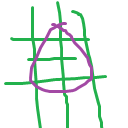
\includegraphics[width=\VAR{geometry.picbox_half_width|round(2)}mm]{pic01}
\caption{}}
\hfill
\parbox[t]{\VAR{geometry.picbox_half_width|round(2)}mm}{
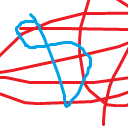
\includegraphics[width=\VAR{geometry.picbox_half_width|round(2)}mm]{pic02}
\caption{}}
\end{figure}
\end{boxedminipage}
\end{boxedminipage}
\begin{boxedminipage}{\VAR{geometry.textwidth|round(2)}mm}
\centering
\smalltitle{设备开机描述}
\begin{boxedminipage}[t]{\VAR{geometry.intro_width|round(2)}mm}
\begin{enumerate}
\BLOCK{for i in 设备开机描述}
\item \VAR{i}
\BLOCK{endfor}
\end{enumerate}
\end{boxedminipage}
\hfill
\begin{boxedminipage}[t]{\VAR{geometry.picbox_width|round(2)}mm}
图片2
\end{boxedminipage}
\end{boxedminipage}
\end{document}